\documentclass[twoside,twocolumn]{article}

\usepackage{blindtext} % Package to generate dummy text throughout this template 

\usepackage[sc]{mathpazo} % Use the Palatino font
\usepackage[T1]{fontenc} % Use 8-bit encoding that has 256 glyphs
\linespread{1.05} % Line spacing - Palatino needs more space between lines
\usepackage{microtype} % Slightly tweak font spacing for aesthetics

\usepackage[english]{babel} % Language hyphenation and typographical rules

\usepackage[hmarginratio=1:1,top=32mm, left=15truemm, right=15truemm, columnsep=20pt]{geometry} % Document margins
\usepackage[hang, small,labelfont=bf,up,textfont=it,up]{caption} % Custom captions under/above floats in tables or figures
\usepackage{booktabs} % Horizontal rules in tables

\usepackage{lettrine} % The lettrine is the first enlarged letter at the beginning of the text

\usepackage{enumitem} % Customized lists
\setlist[itemize]{noitemsep} % Make itemize lists more compact

\usepackage{abstract} % Allows abstract customization
\renewcommand{\abstractnamefont}{\normalfont\bfseries} % Set the "Abstract" text to bold
\renewcommand{\abstracttextfont}{\normalfont\small\itshape} % Set the abstract itself to small italic text

\usepackage{titlesec} % Allows customization of titles
\usepackage{graphicx}
\renewcommand\thesection{\Roman{section}} % Roman numerals for the sections
\renewcommand\thesubsection{\roman{subsection}} % roman numerals for subsections
\titleformat{\section}[block]{\large\scshape\centering}{\thesection.}{1em}{} % Change the look of the section titles
\titleformat{\subsection}[block]{\large}{\thesubsection.}{1em}{} % Change the look of the section titles

\usepackage{fancyhdr} % Headers and footers
\pagestyle{fancy} % All pages have headers and footers
\fancyhead{} % Blank out the default header
\fancyfoot{} % Blank out the default footer
\fancyhead[C]{Running title $\bullet$ May 2016 $\bullet$ Vol. XXI, No. 1} % Custom header text
\fancyfoot[RO,LE]{\thepage} % Custom footer text

\usepackage{titling} % Customizing the title section

\usepackage{hyperref} % For hyperlinks in the PDF
\usepackage{algorithm, algorithmic}
\usepackage{amsmath}
\usepackage{bm}
\renewcommand{\algorithmicrequire}{\textbf{Input:}}
\renewcommand{\algorithmicensure}{\textbf{Output:}}
\newcommand{\argmax}{\mathop{\rm arg~max}\limits}
\newcommand{\argmin}{\mathop{\rm arg~min}\limits}
\newcommand{\E}{\mathbb{E}}
%----------------------------------------------------------------------------------------
%	TITLE SECTION
%----------------------------------------------------------------------------------------

\setlength{\droptitle}{-4\baselineskip} % Move the title up

\pretitle{\begin{center}\Huge\bfseries} % Article title formatting
\posttitle{\end{center}} % Article title closing formatting
\title{Project Report EEC264} % Article title
\author{Toshinori Kitamura}
\date{\today} % Leave empty to omit a date
\renewcommand{\maketitlehookd}{%
% \begin{abstract}
% \noindent 
% \end{abstract}
}

%----------------------------------------------------------------------------------------

\begin{document}
\setlength{\abovedisplayskip}{0.5pt}
\setlength{\belowdisplayskip}{0.5pt}

\maketitle
\section{Introduction\label{introduction}}

This report explains about a paper "Optimal Bayesian Kalman Filtering with Prior Update"\cite{Dehghannasiri2018}. 
The optimal bayesian Kalman Filter(OBKF) is an advanced version of the intrinsically bayesian robust Kalman filter(IBRKF)\cite{Dehghannasiri2017}, which is a Kalman filter exploiting the prior knowledge for the model.

The Kalman filter(classic KF)\cite{Kalman1960} is a widely used technique to estimate the state vector of a linear dynamics system from its previous estimation and the measurement. Although it provides the best estimation in some condition, it has a problem. 
That is, the classic KF is highly sensitive to the noise covariance of the target linear dynamic system\cite{Sangsuk-Iam1990}. To manage this problem, mainly two robust approaches, bayesian approach and non-bayesian approach, have been studied. 

The adaptive Kalman filter\cite{Myers1976}\cite{Mehra1972} is a non-bayesian approach to achieve the robustness towards the uncertain system. It achieves the robustness by estimating the covariance matrixes during the state estimation. Although it doesn't require any prior knowledge, it needs a lot of observation data to tune the parameter. For a certain problem like gene regulatory network, the cost to obtain the data is expensive, so algorithms which doesn't require a lot of data are preferred.

On the other hand, because of its prior knowledge, the bayesian approach doesn't require so many data comared with non-bayesian approaches. The bayesian approach Kalman filter, IBRKF, is robust in the sense of that it minimizes the average MSE relative to the prior distribution. 

The IBRKF achieves the robustness in bayesian sense, but it doesn't utilizes the any information obtained from the observation. The OBKF exploits the both prior knowledge and the observation data, and it achieves the optimal estimation relative to the posterior distribution.

The rest of this paper is organized as follows. Section \ref{sec: kf} explains the overview of the classic Kalman filter and its problem. In section \ref{sec: ibr}, a bayesian approach, IBR Kalman filter is explained. Section \ref{sec: obkf} describes the OBKF, and section \ref{sec:performance} shows the simulated results and the performance of the OBKF. Finally, section \ref{sec:conclusion} summerizes the OBKF.
\section{Kalman filter\label{sec: kf}}

The classic KF is the optimal linear estimator for linear dynamic systems. A linear dynamic system is written as

\begin{align}
{\bf x}_{k+1} &= \bm{\Phi}_k{\bf x}_{k} + \bm{\Gamma}_k{\bf u}_{k}\\
{\bf y}_{k} &= {\bf H}_k{\bf x}_{k} + {\bf v}_{k}
\end{align}

Where, 
\begin{itemize}
    \item ${\bf x}_k$: {\it state vector}
    \item ${\bf y}_k$: {\it observation vector}
    \item ${\bf u}_k$, ${\bf v}_k$: {\it zero-mean gaussian noise vector}
    \item $\bm{\Phi}_k, \; \bm{\Gamma}_k, \; \bm{H}_k$: {\it transition matrix}
\end{itemize}

And the noise statistics are:

\begin{align}
    \E[{\bf u}_k{\bf u}_l^T]&={\bf Q}\delta_{kl},\;
    \E[{\bf v}_k{\bf v}_l^T]={\bf R}\delta_{kl},\; \forall k,l=0,1,...\\
    \E[{\bf v}_k{\bf x}_l^T]&={\bf 0},\;\;\;\;\;\;
    \E[{\bf u}_k{\bf v}_l^T]={\bf 0}\; \forall k,l=0,1,...\\
    \E[{\bf u}_k{\bf y}_l^T]&={\bf 0}, \;\; 0\leq l\leq k,
\end{align}

For such linear dynamic systems, the classic KF provides the linear estimation $\bm{\hat x}_k$ minimizing the mean squared error based on the observations $\bm{y}_l$, $l\leq k-1$. The estimated state vector is given as,

\begin{equation} \label{eq:cost}
    \bm{\hat x}_k = \argmin_{\bm{\hat x}_k}\E[|\bm{x}_k-\bm{\hat x}_k|^2]
\end{equation}

Let the mean of the estimated $\bm{\hat x}_k$ be itself $\bm{\hat x}_k$ and the covariance of it be as ${\bf P^x}_{k}$. Then, the classic KF algorithm is obtained by the Algorithm \ref{al:KF}.

\begin{algorithm}[H]
\caption{Classic Kalman Filter}
\begin{algorithmic}[1]
\label{al:KF}
\REQUIRE ${\bf \hat x}_k$, ${\bf P^x}_{k}$, ${\bf y}_k$
\STATE $\tilde {\bf z}_k = {\bf y}_k - {\bf H}_k{\bf \hat x}_k$
\STATE ${\bf K}_k = {\bf P^x}_k{\bf H}^T_k({\bf H}_k{\bf P^x}_k{\bf H}^T_k+{\bf R})^{-1}$
\STATE $\hat{\bf x}_{k+1} = \bm{\Phi}_k{\bf \hat x}_k+\bm{\Phi}_k{\bf K}_k{\bf \tilde z}_k$
\STATE ${\bf P^x}_{k+1} = \bm{\Phi}_k({\bf I}-{\bf K}_k{\bf H}_k){\bf P^x}_k\bm{\Phi}^T_k + \bm{\Gamma}_k{\bf Q}\bm{\Gamma}_k^T$
\ENSURE ${\bf \hat x}_{k+1}$, ${\bf P^x}_{k+1}$
\end{algorithmic}
\end{algorithm}

This algorithm minimizes the (\ref{eq:cost}), but it has a problem. This algorithm provides poor estimation if the covariance matrix ${\bf Q}$ and ${\bf R}$ is very different from the exact value. Therefore, a robust method is required to manage this problem.
\section{IBR Kalman Filter\label{sec: ibr}}

The IBRKF is a robust Kalman filter exploiting the prior knowledge. To begin with, suppose the noise covariance are expressed by unknown parameter vector $\bm{\theta}=[\theta_1, \theta_2]$. It is governed by the prior distribution $\pi(\bm{\theta})$, and the noise statistics is written as
\begin{align}
    \E[{\bf u}^{\theta_1}_k ({\bf u}^{\theta_1}_l)^T]={\bf Q}^{\theta_1}\delta_{kl} \\
    \E[{\bf v}^{\theta_2}_k ({\bf v}^{\theta_2}_l)^T]={\bf R}^{\theta_2}\delta_{kl} 
\end{align}

The IBRKF is robust in the sense of that it minimizes the cost function (\ref{eq:cost}) relative to the prior distribution. That means, the IBRKF produces the $\bm{\hat x}_k$ given as

\begin{equation} \label{eq:ibrcost}
    \bm{\hat x}_k = \argmin_{\bm{\hat x}_k}\E_{\bm{\theta}}[\E[|\bm{x}_k-\bm{\hat x}_k|^2]]
\end{equation}

The algorithm which provides (\ref{eq:ibrcost}) is similar to the one of classic KF. It's obtained by the Algorithm \ref{al:IBR}.

\begin{algorithm}[]
\caption{IBR Kalman Filter}
\begin{algorithmic}[1]
    \label{al:IBR}
\REQUIRE ${\bf \hat x}^{\bm{\theta}}_k$, $\E_{\bm{\theta}}[{\bf P}^{\bm{x, \theta}}_{k}]$, ${\bf y}^{\bm{\theta}}_k$
\STATE $\tilde {\bf z}^{\bm{\theta}}_k = {\bf y}^{\bm{\theta}}_k - {\bf H}_k{\bf \hat x}^{\bm{\theta}}_k$
\STATE ${\bf K}^{\Theta}_k = \E_{\bm{\theta}}[{\bf P}^{\bm{x, \theta}}_k]{\bf H}^T_k\E_{\bm{\theta}}^{-1}[{\bf H}_k{\bf P}^{\bm{x, \theta}}_k{\bf H}^T_k+{\bf R}^{\bm{\theta_2}}]$
\STATE $\hat{\bf x}^{\bm{\theta}}_{k+1} = {\Phi}_k{\bf \hat x}^{\bm{\theta}}_k+{\Phi}_k{\bf K}^{\bm{\Theta}}_k{\bf \tilde z}^{\bm{\theta}}_k$
\STATE $\E_{\bm\theta}[{\bf P}^{\bm{x, \theta}}_{k+1}] = {\Phi}_k({\bf I}-{\bf K}^{\Theta}_k{\bf H}_k)\E_{\bm\theta}[{\bf P}^{\bm{x, \theta}}_k]{\Phi}^T_k + {\Gamma}_k\E_{\theta_1}[{\bf Q}^{\theta_1}_k]{\Gamma}_k^T$
\ENSURE ${\bf \hat x}^{\bm{\theta}}_{k+1}$, $\E_{\bm\theta}[{\bf P}^{\bm{x, \theta}}_{k+1}]$
\end{algorithmic}
\end{algorithm}

It's worth nothing that the IBR Kalman Filter is obtained just replacing ${\bf Q}$ and ${\bf R}$ in Classic Kalman Filter with $\E_{\theta_1}[{\bf R}^{\theta_1}]$ and $\E_{\theta_2}[{\bf Q}^{\theta_2}]$ respectively. Since the covariance matrixes are same during the algorithm, the computational cost is exactly same as the classic KF. 

\section{Prior update: Optimal Bayesian Kalman Filter}

\begin{frame}
    \tableofcontents[currentsection]
\end{frame}

\subsection{Basic Idea}
\begin{frame}{Basic Idea: OBKF}
    \begin{itemize}
        \item Based on the IBR Kalman Filter
        \item Utilize measured data $\mathcal{Y}_{k}=\{{\bf y}_0,...,{\bf y}_{k}\}$to obtain the posterior distribution $\pi(\theta|\mathcal{Y}_k)$
        \item Best estimation relative to $\pi(\theta|\mathcal{Y}_{k-1})$: $\argmin_{{\bf \hat x_\theta}(k)} E_\theta[E[({\bf x_\theta}(k) - {\bf \hat x_\theta}(k))^T\times ({\bf x_\theta}(k) - {\bf \hat x_\theta}(k))]|\mathcal{Y}_{k-1}]$
    \end{itemize}
\end{frame}


\subsection{Algorithm}
\begin{frame}{Algorithm: OBKF}
\begin{itemize}
    \item OBKF is obtained just replacing ${\bf Q}$ and ${\bf R}$ in Classic Kalman Filter with $E_{\theta_1}[{\bf Q^{\theta_1}}|\mathcal{Y}_k]$ and $E_{\theta_1}[{\bf R^{\theta_2}}|\mathcal{Y}_k]$ respectively
\end{itemize}
\begin{algorithm}[H]
\caption{OBKF}
\begin{algorithmic}[1]
\REQUIRE ${\bf \hat x}^{\theta}_k$, $E_\theta[{\bf P^{x, \theta}}_{k}|\mathcal{Y}_{k-1}]$, $\mathcal{Y}_k$
\STATE $\tilde {\bf z}^{\bf \theta}_k = {\bf y}^{\bf \theta}_k - {\bf H}_k{\bf \hat x}^{\bf \theta}_k$
\STATE ${\bf K}^{\bf \Theta^*}_k = E_\theta[{\bf P^{x, \theta}}_k|\mathcal{Y}_{k-1}]{\bf H}^T_kE_\theta^{-1}[{\bf H}_k{\bf P^{x, \theta}}_k{\bf H}^T_k+{\bf R^{\theta_2}}|\mathcal{Y}_{k-1}]$
\STATE $\hat{\bf x}^{\theta}_{k+1} = {\bf \Phi}_k{\bf \hat x}^{\theta}_k+{\bf \Phi}_k{\bf K}^{\bf \Theta}_k{\bf \tilde z}^{\theta}_k$
\STATE $E_\theta[{\bf P^{x, \theta}}_{k+1}|\mathcal{Y}_k] = {\bf \Phi}_k({\bf I}-{\bf K}^{\bf \Theta^*}_k{\bf H}_k)E_\theta[{\bf P^{x, \theta}}_k|\mathcal{Y}_k]{\bf \Phi}^T_k + {\bf \Gamma}_kE_{\theta_1}[{\bf Q^{\theta_1}}|\mathcal{Y}_k]{\bf \Gamma}_k^T$
\ENSURE ${\bf \hat x}^{\theta}_{k+1}$, $E_\theta[{\bf P^{x, \theta}}_{k+1}|\mathcal{Y}_{k}]$
\end{algorithmic}
\end{algorithm}

\pause

How are the posterior expectations found: $E_{\theta_1}[{\bf Q^{\theta_1}}|\mathcal{Y}_k]$ and $E_{\theta_2}[{\bf R^{\theta_2}}|\mathcal{Y}_k]$ ?

\end{frame}

\subsection{Find Posterior Expectations}
\begin{frame}{Find Posterior Expectatoins: $E_{\theta_1}[{\bf Q^{\theta_1}}|\mathcal{Y}_k]$ and $E_{\theta_2}[{\bf R^{\theta_2}}|\mathcal{Y}_k]$}
\begin{itemize}
    \item Approximate $E_{\theta_1}[{\bf Q^{\theta_1}}|\mathcal{Y}_k]$ and $E_{\theta_2}[{\bf R^{\theta_2}}|\mathcal{Y}_k]$ using Metropolis Hastings MCMC
    \item MCMC requires the likelihood function $f(\mathcal{Y}_k|\theta)$
    \item $f(\mathcal{Y}_k|\theta)$ is calculated by:
    \begin{itemize}
        \item Marginalize $f(\mathcal{Y}_k, \mathcal{X}_k|\theta)$ over $\mathcal{X}_k$
        \item Factorize $f(\mathcal{Y}_k, \mathcal{X}_k|\theta)$ by the Markov assumption
        \item Using the factor-graph, this step can be simplified 
        \item $f(\mathcal{Y}_k|\theta)$ can be calculated by recursive algorithm
    \end{itemize}
\end{itemize}
\end{frame}

\begin{frame}{Algorithm: Likelihood Function Calculation}

\begin{algorithm}[H]
\caption{Factor-Graph-Based Likelihood Function Calculation}
\begin{algorithmic}[1]
\REQUIRE $\theta$, $\mathcal{Y}_k$
\STATE ${\bf M}_0 \leftarrow E[{\bf x}_0],\; S_0 \leftarrow 1,\; {\bf \Sigma}_0 \leftarrow cov[{\bf x}_0], \; i \leftarrow 0$
\WHILE {$i \leq k-1$}
    \STATE ${\bf W}_i\leftarrow {\bf H}_i^T({\bf R}^{\theta_2})^{-1}{\bf y}_i + {\bf \Sigma}_i^{-1}{\bf M}_i$
    \STATE ${\bf \Lambda}_i^{-1}\leftarrow {\bf \Phi}_i^T({\bf \tilde Q}_i^{\theta_1})^{-1}{\bf \Phi}_i + {\bf H}_i^{T}({\bf R}^{\theta_2})^{-1}{\bf H}_i+{\bf \Sigma}_i^{-1}$
    \STATE ${\bf \Sigma}_{i+1}^{-1}\leftarrow ({\bf \tilde Q}_i^{\theta_1})^{-1} - ({\bf \tilde Q}_i^{\theta_1})^{-1}{\bf \Phi}_i{\bf \Lambda}_i{\bf \Phi}_i^T({\bf \tilde Q}_i^{\theta_1})^{-1}$
    \STATE ${\bf M}_{i+1}\leftarrow {\bf \Sigma}_{i+1}({\bf \tilde Q}_i^{\theta_1})^{-1}{\bf \Phi_i}{\bf \Lambda}_i({\bf H}_i^T({\bf R}^{\theta_2})^{-1}{\bf y}_i+{\bf \Sigma}_i^{-1}{\bf M}_i)$
    \STATE $S_{i+1} \leftarrow \text{using Eq.(29) in the paper}$
    \STATE $i \leftarrow i+1$
\ENDWHILE
\STATE ${\bf \Delta}_k^{-1}\leftarrow {\bf H}_k^T({\bf R}^{\theta_2})^{-1}{\bf H}_k + {\bf \Sigma}_k^{-1}$
\STATE ${\bf G}_k \leftarrow {\bf \Delta}_k({\bf H}_k^T({\bf R}^{\theta_2})^{-1}{\bf y}_k + {\bf \Sigma}_k^{-1}{\bf M}_k)$
\STATE $f(\mathcal{Y}_k|\theta) \leftarrow \text{using Eq.(34) in the paper}$
\ENSURE $f(\mathcal{Y}_k|\theta)$
\end{algorithmic}
\end{algorithm}
\end{frame}

\subsection{Performance}

\begin{frame}{Performance: Accuracy}
% Good image will inserted here
% Bigger figure
\pnote{
    * figureはtheta1=1, theta2=knownの時のlocalizationについてのシミュレーション結果を示している。
    * figureは各カルマンフィルタの精度を示している。縦軸が精度と同じだと思ってくれて構わない。黒線はtheta1=1を使用したクラシックカルマンフィルタであり、これ以上の精度は出すことは出来ない。図より、OBKFは他の手法と比較して最も早く最適なカルマンフィルタにconvergeしていることがわかる。
}
\begin{figure}[H]
    \begin{center}
    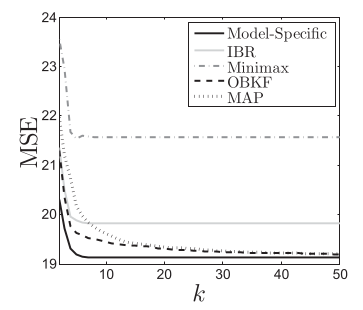
\includegraphics[width=7cm]{img/OBKF_r1.png}
    \caption{Performance analysis for specific $\theta_1 = 1$ and known $\theta_2$  \protect\linebreak OBKF achieves the lowest MSE (cited from \cite{Dehghannasiri2018})}
    \label{fig:r_1}
    \end{center}
\end{figure}
\end{frame}

\begin{frame}{Performance: Data Efficiency}
    \pnote{
    * figureはthetaがunknownであるときに高いMSEを達成するのに必要なstep数kを示している。
    }
\begin{figure}[H]
    \begin{center}
    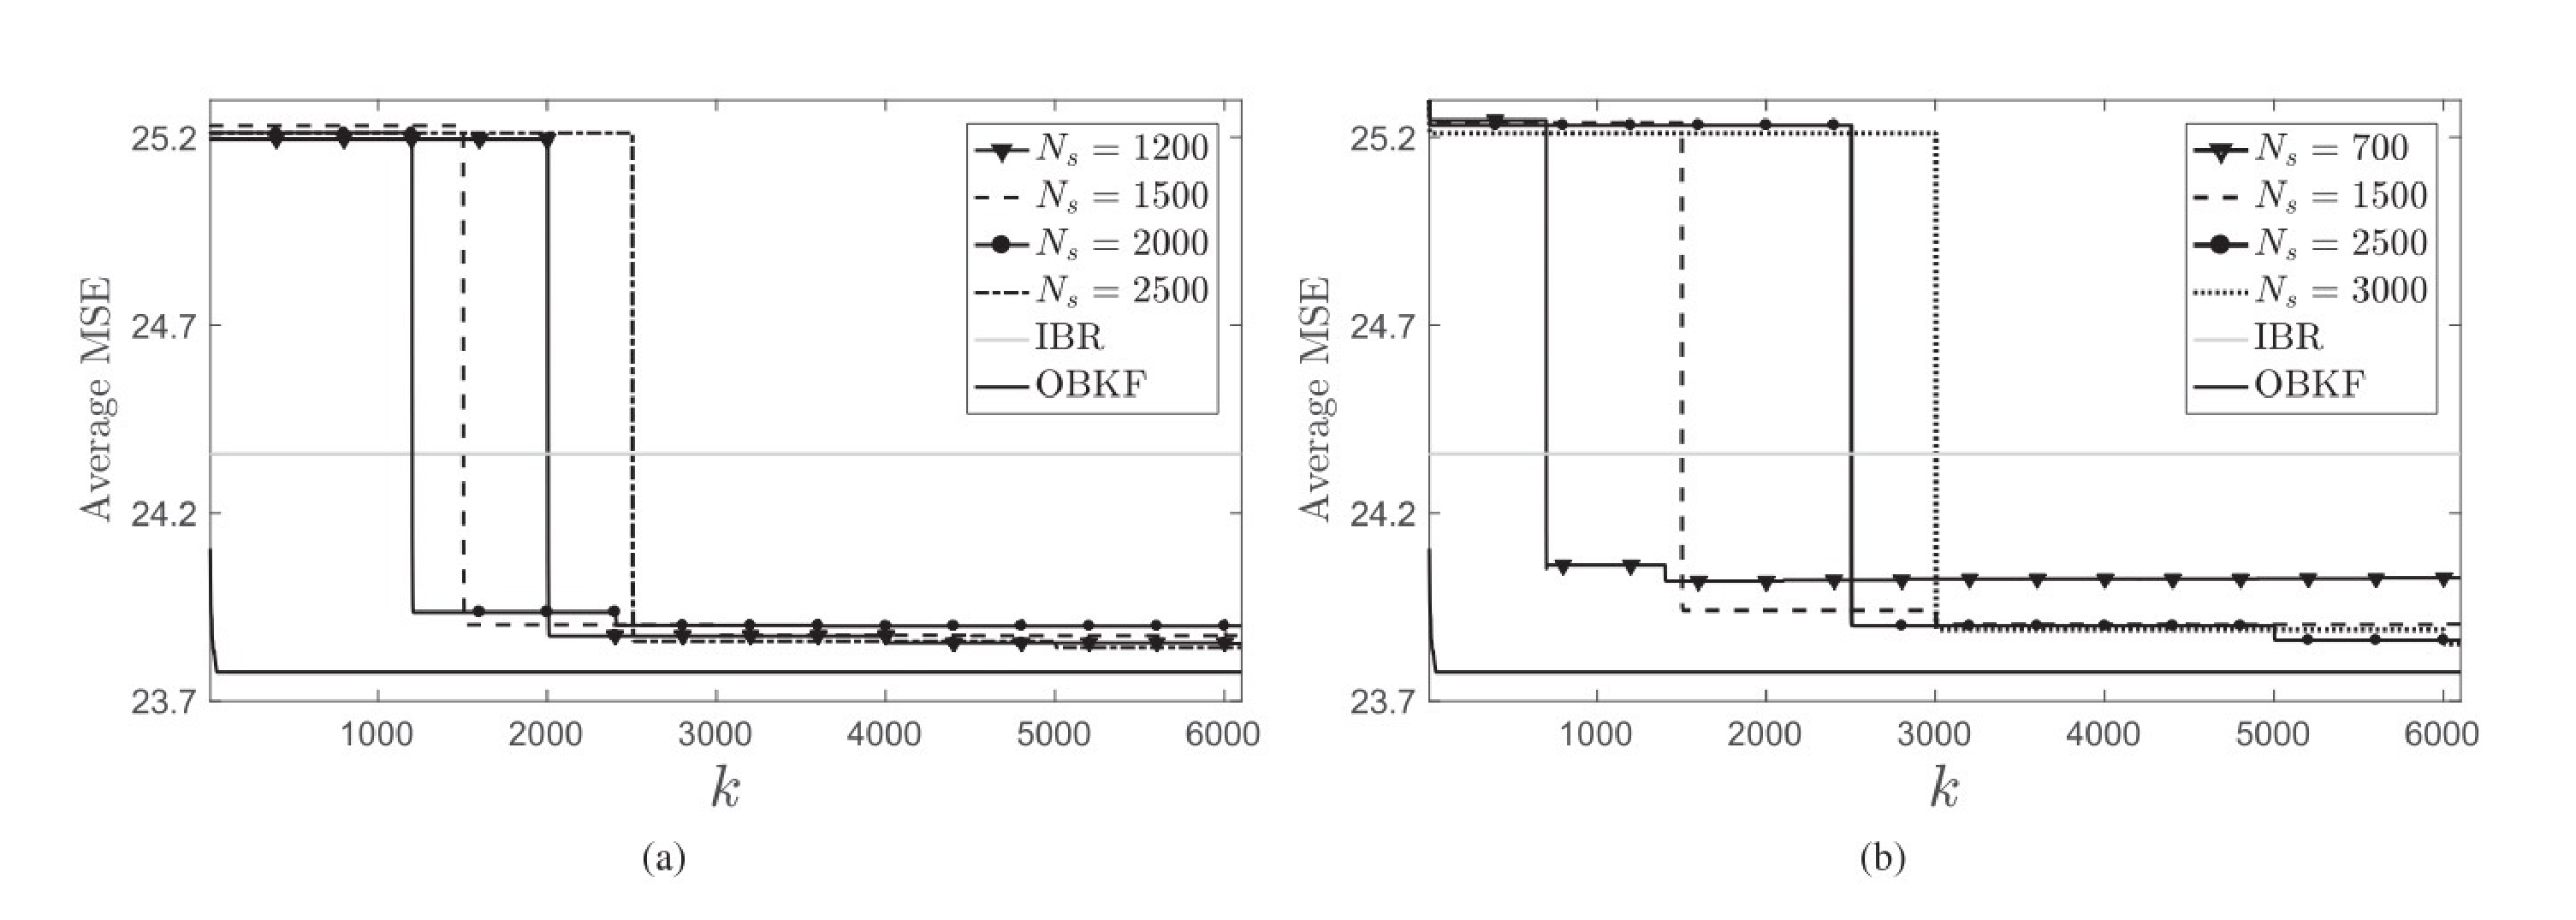
\includegraphics[width=9cm]{img/cmp_adaptive.eps}
    \caption{Unknown $\theta_1$ and comparison with an adaptive Kalman Filter (cited from \cite{Dehghannasiri2018})}
    \label{fig:cmp_adaptive}
    \end{center}
\end{figure}

\end{frame}


\subsection{Problems and Future Works}
\begin{frame}{Problems and Future Works}
\begin{itemize}
    \item If the prior distribution doesn't include the true value, the estimation won't converge
    \item Factor-graph and MCMC are computationally expensive. Finding an efficient approach is a future work.
\end{itemize}
\end{frame}
\section{Simulation and Performance}\label{sec:performance}

The author compares the OBKF with the model specific Kalman filter, IBRKF, minimax Kalman filter, and MAP Kalman filter. The model specific Kalman filter is the classic KF with true unknown parameter. The minimax Kalman filter provides the best worst case performance. The MAP Kalman filter is the classic KF with the MAP estimates of the unknown parameter. 
To evaluate the estimation, the covariance of the estimation error is used. In the equation (\ref{eq:metric}), ${\bf P^x}_{k+1}(\bm{\theta};\bm{\theta}')$ is the covariance of the estimation error $\bm{x}_k-\bm{\hat x}_k$. 

\begin{align}\label{eq:metric}
{\bf P^x}_{k+1}(\bm{\theta};\bm{\theta}') &= \bm{\Phi}_k({\bf I}-{\bf K}^{\bm{\theta}'}_k{\bf H}_k){\bf P^x}_k(\bm{\theta};\bm{\theta}')({\bf I}-{\bf K}^{\bm{\theta}'}_k{\bf H}_k)^T\bm{\Phi}^T_k \nonumber \\
&\quad + \bm{\Gamma}_k{\bf Q}^{\theta_1}\bm{\Gamma}_k^T + \bm{\Phi}_k\bm{K}_k^{\bm{\theta}'}\bm{R}^{\theta_2}(\bm{K}_k^{\bm{\theta}'})^T\bm{\Phi}_k^T
\end{align}

The trace of ${\bf P^x}_{k+1}(\bm{\theta};\bm{\theta}')$ is computed as the MSE of the estimation, and it is used as the metric.

To evaluate the performance of the OBKF, consider a 2-D tracking problem with an unknown parameter. In the problem, the state vector is $\bm{x}_k=[p_x\, v_x\, p_y\, v_y]^T$, where $p_x,\, v_x,\, p_y,\, v_y$ are the position and velocity of the x and y dimmensions, respectively. The parameters in the (\ref{eq:linear1}) and (\ref{eq:linear2}) are given as follows.

\begin{align*}
    &\bm{\Phi}_k=
    \begin{bmatrix}
        1 & \tau & 0 & 0\\
        0 & 1 & 0 & 0 \\
        0 & 0 & 1 & \tau \\
        0 & 0 & 0 & 1 \\
    \end{bmatrix}, \;\;
    \bm{H}_k = 
    \begin{bmatrix}
        1&0&0&1\\
        0&0&1&0
    \end{bmatrix}, \;\;
    \bm{\Gamma}_k = \bm{I} \\
    &\bm{Q} = q \times 
    \begin{bmatrix}
        \tau^3/3 & \tau^2/2 & 0 & 0 \\
        \tau^2/2 & \tau & 0 & 0 \\
        0 & \tau & 0 & 0 \\
        0 & 0 & \tau^2/2 & \tau
    \end{bmatrix}, \;\;
    \bm{R}=r\times\begin{bmatrix}
        1&0\\
        0&1
    \end{bmatrix}
\end{align*}

Here, $\tau$ is the measurement interval. $q$ and $r$ are the covariance noise intensity.

In the simulation, the author uses $\tau = 1$ second. The initial conditions are set as $\E[\bm{x}_0]=[100\, 10\, 30\, -10]^T$ and ${\rm cov}[\bm{x}_0]={\rm diag}([25\, 2\, 25\, 2])$ where ${\rm diag}(v)$ is a diagonal matrix whose diagonal elements are $v$.
The parameter $q$ is set to 2 and $r$ is defined as a random variable, uniformly distributed over [0.25,4]. 

\begin{figure}[H]
    \begin{center}
    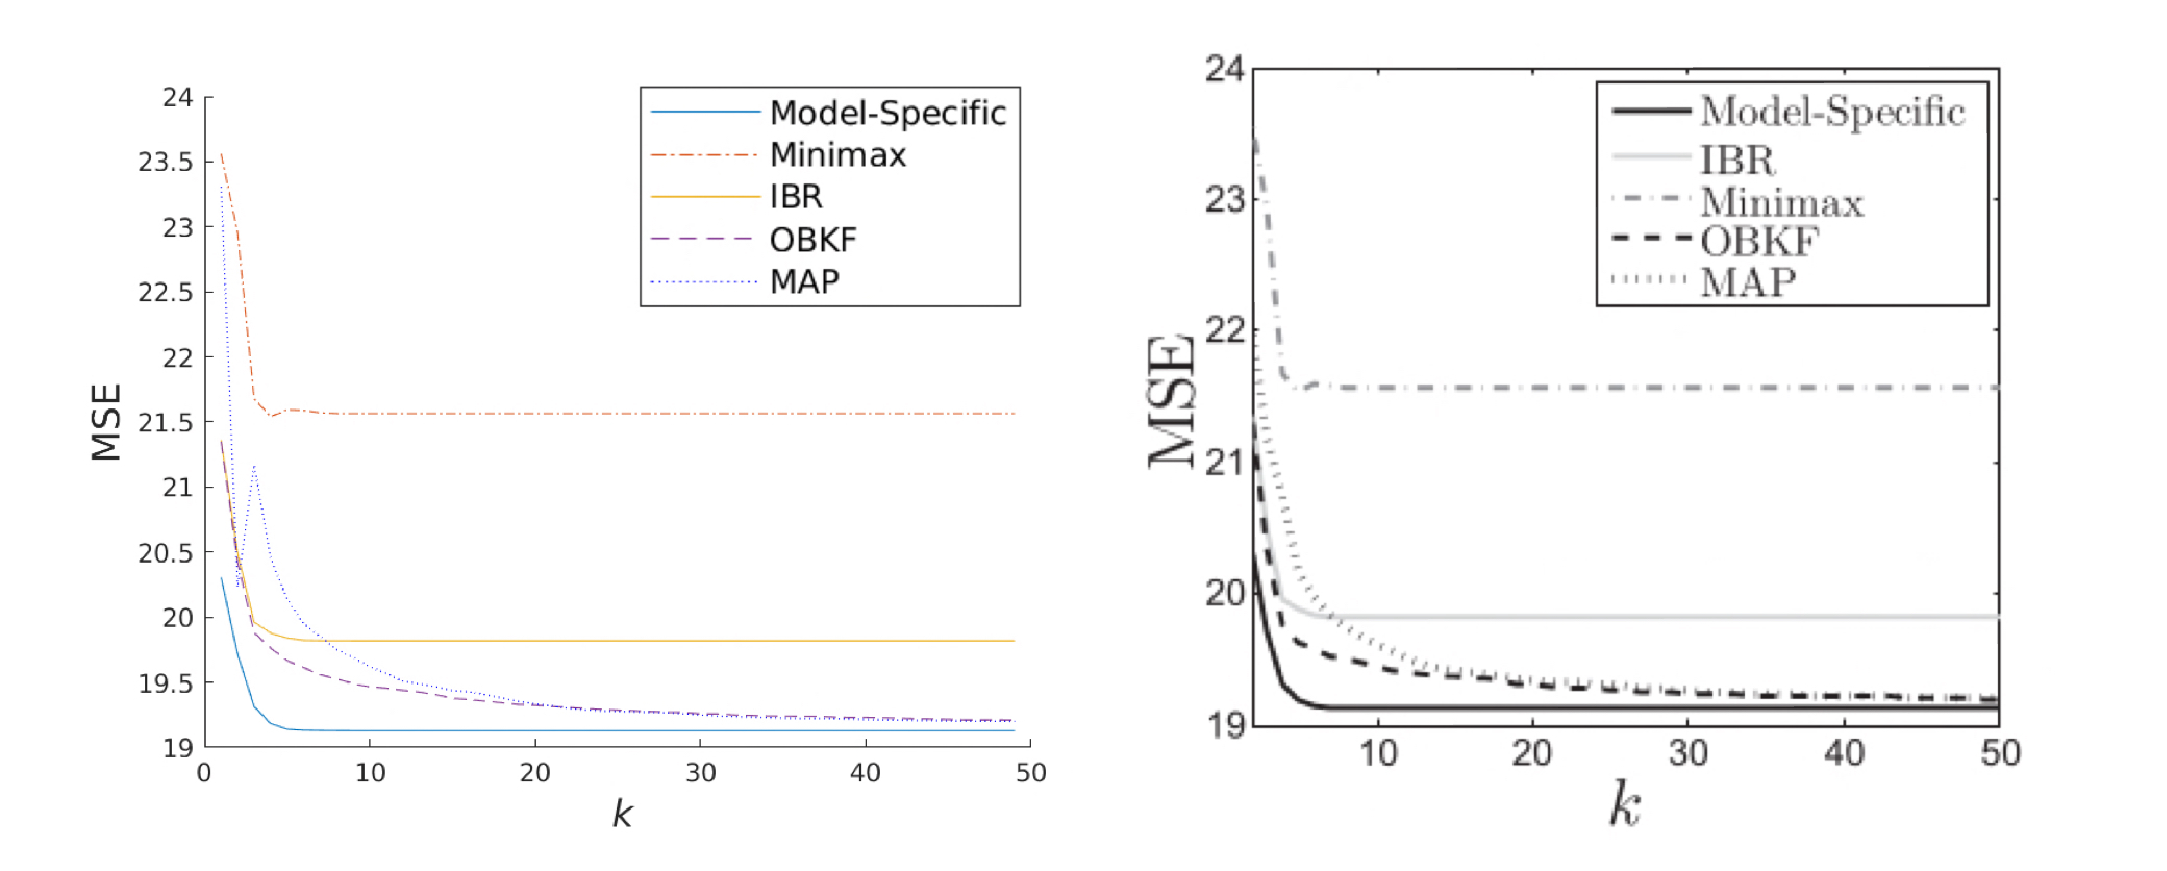
\includegraphics[width=9.7cm]{img/r1_mse.eps}
    \caption{MSE for $r=1$. The left figure shows the result simulated on my laptop. Right figure is cited from the OBKF paper\cite{Dehghannasiri2018}.}
    \label{fig:mse_r1}
    \end{center}
\end{figure}
\begin{figure}[H]
    \begin{center}
    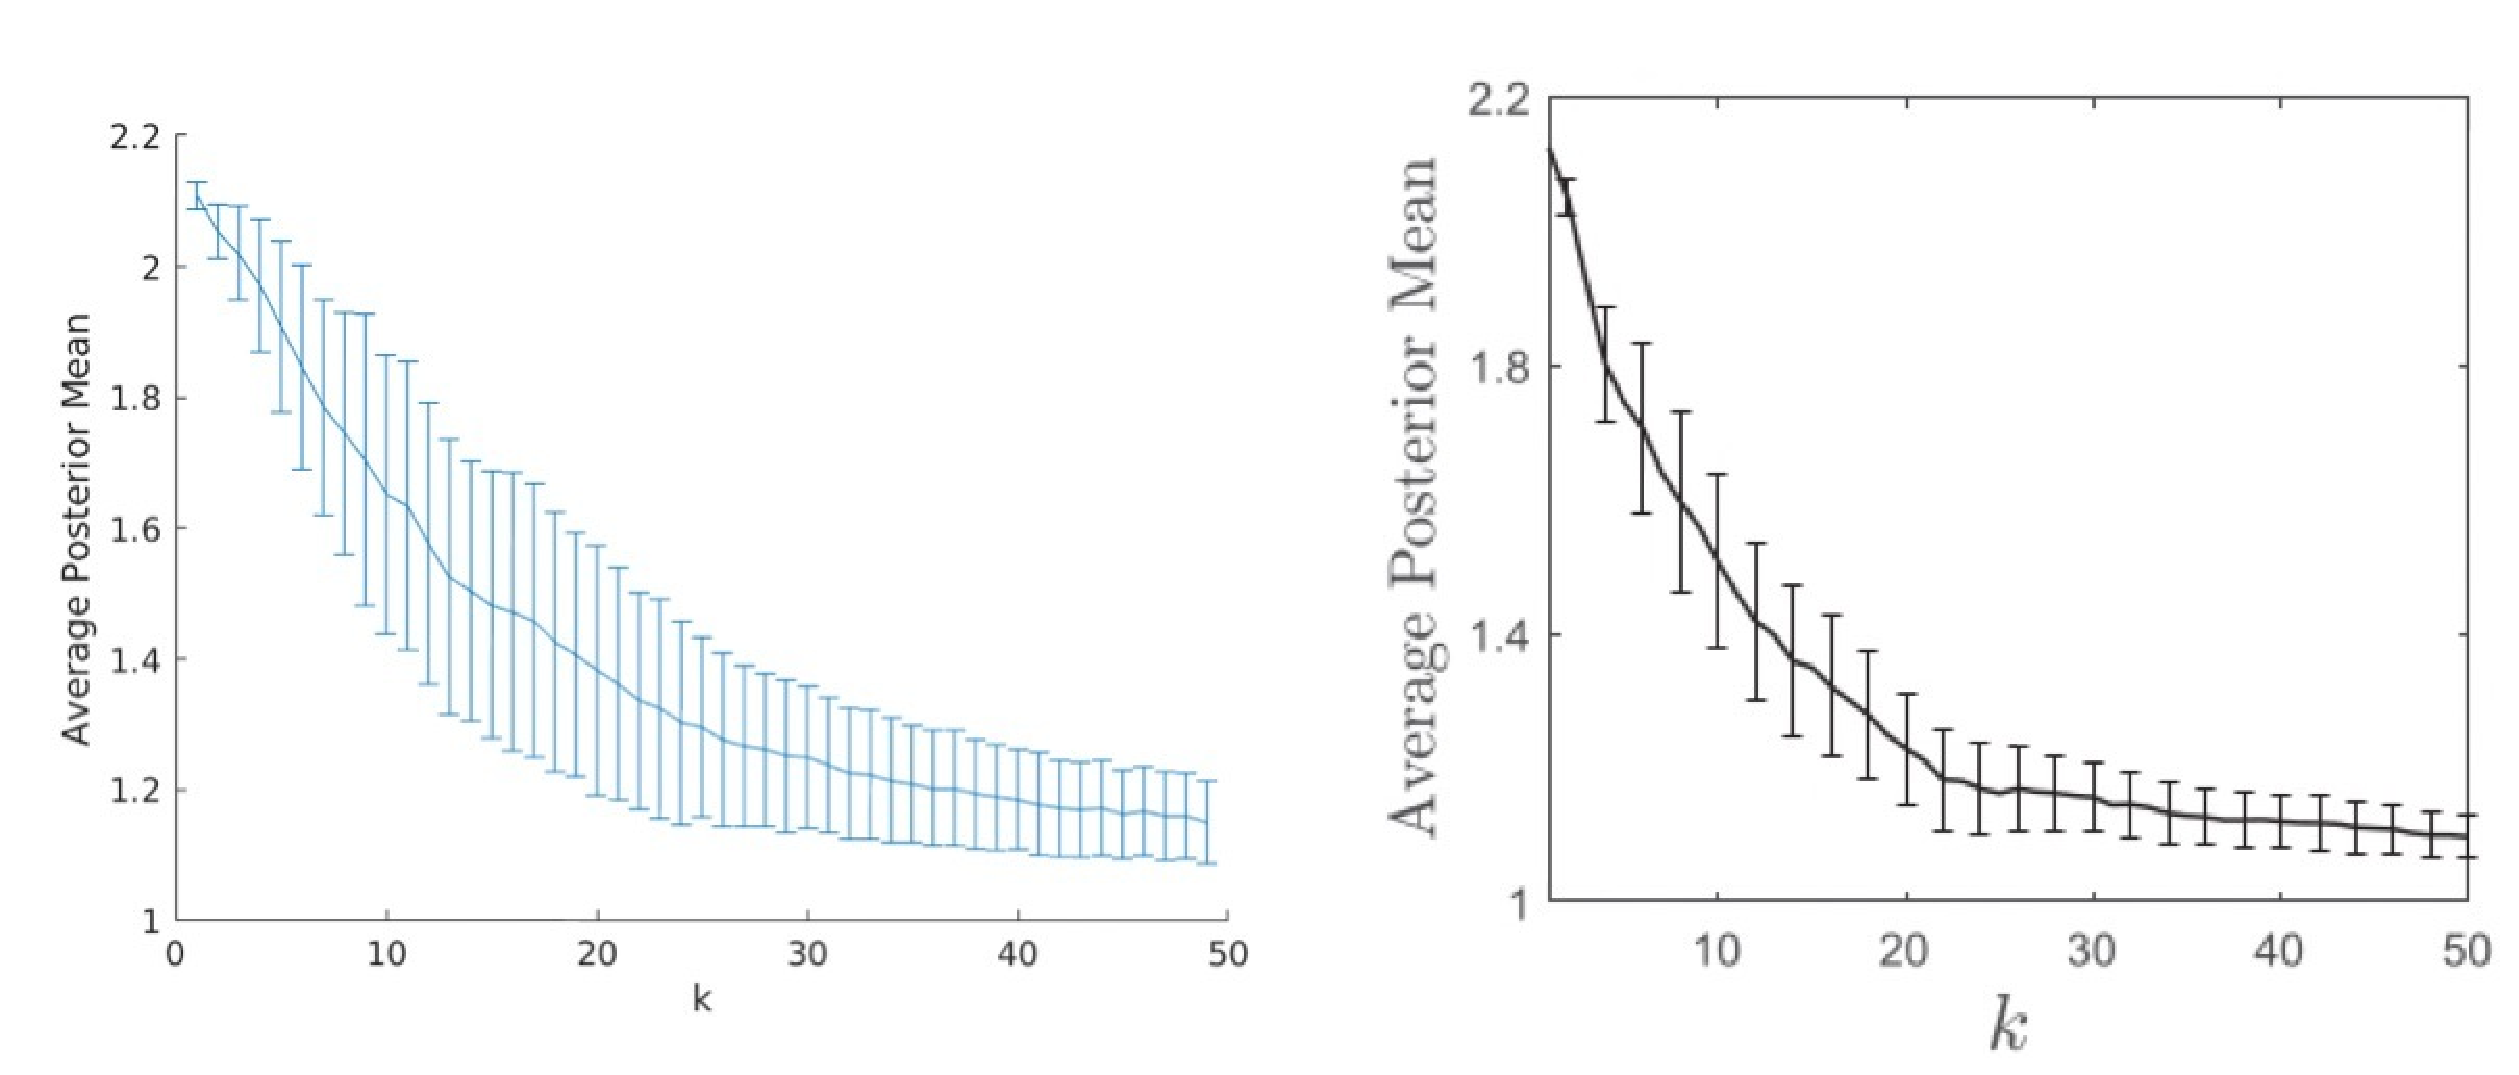
\includegraphics[width=9.7cm]{img/r1_mean.eps}
    \caption{Empirical average and variance of $\E[r|\mathcal{Y}_k]$. The left figure shows the result simulated on my laptop. Right figure is cited from the OBKF paper\cite{Dehghannasiri2018}.}
    \label{fig:mean_r1}
    \end{center}
\end{figure}

From the view of the estimation accuracy, the OBKF achieves the best performance. Fig.\ref{fig:mse_r1} compares the simulated MSE on my laptop with the figure from the paper. You can see that in the both images, the OBKF outperforms the other Kalman filters. The OBKF converges. The OBKF converges the fastest and reaches almost the model-specific KF as $k$ increases. Fig.\ref{fig:mean_r1} compares the estimated $r$ simulated on my laptop and the figure from the paper. In the both image, the estimated $r$ converges to the true value $r=1$ as k increases. That means that the estimation is getting close to the model-specific KF as the $k$ increases.

\begin{figure*}[h]
    \begin{center}
    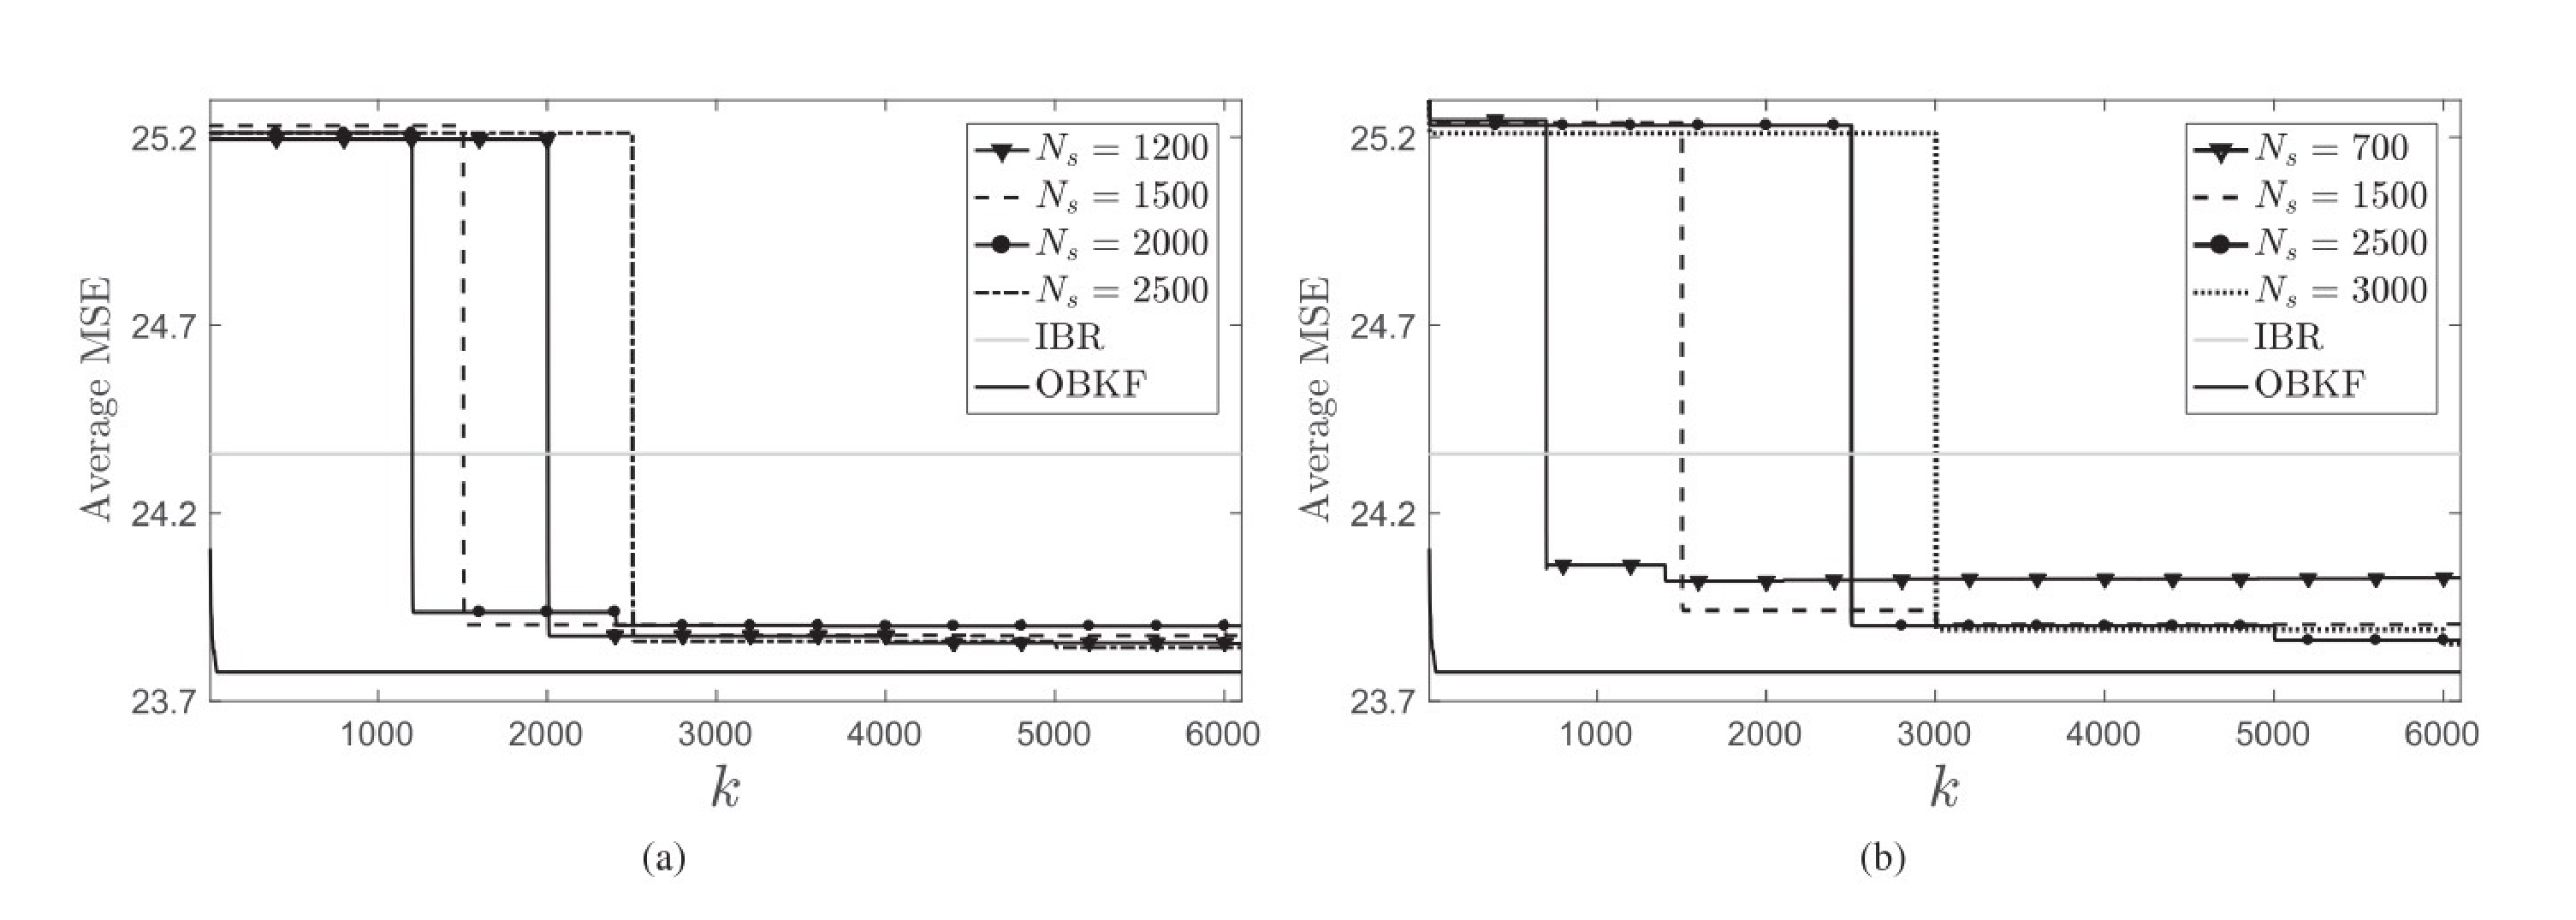
\includegraphics[width=15cm]{img/cmp_adaptive.eps}
    \caption{Comparison with the adaptive Kalman filters. (a) Unknown $r$ and comparison with the Myers method. (b) Unknown $r$ and comparison with the Mehra method. Cited from \cite{Dehghannasiri2018}}
    \label{fig:cmp_adaptive}
    \end{center}
\end{figure*}

Compared with the non-bayesian approach, the OBKF achieves much efficient estimation in the sense of the number of data. Fig.\ref{fig:cmp_adaptive} compares the OBKF and the adaptive Kalman filter with unknown parameter $r$ uniformly distributed over [0.25, 4]. The adaptive methods depend on the parameter $N_s$, which is the number of the observations to tune the filter. If the $N_s$ is small, the adaptive Kalamn filter estimates poorly and can be unstable in the long run. From Fig.\ref{fig:cmp_adaptive}, you can see that the OBKF converges much faster than the adaptive methods.

\begin{figure}[H]
    \begin{center}
    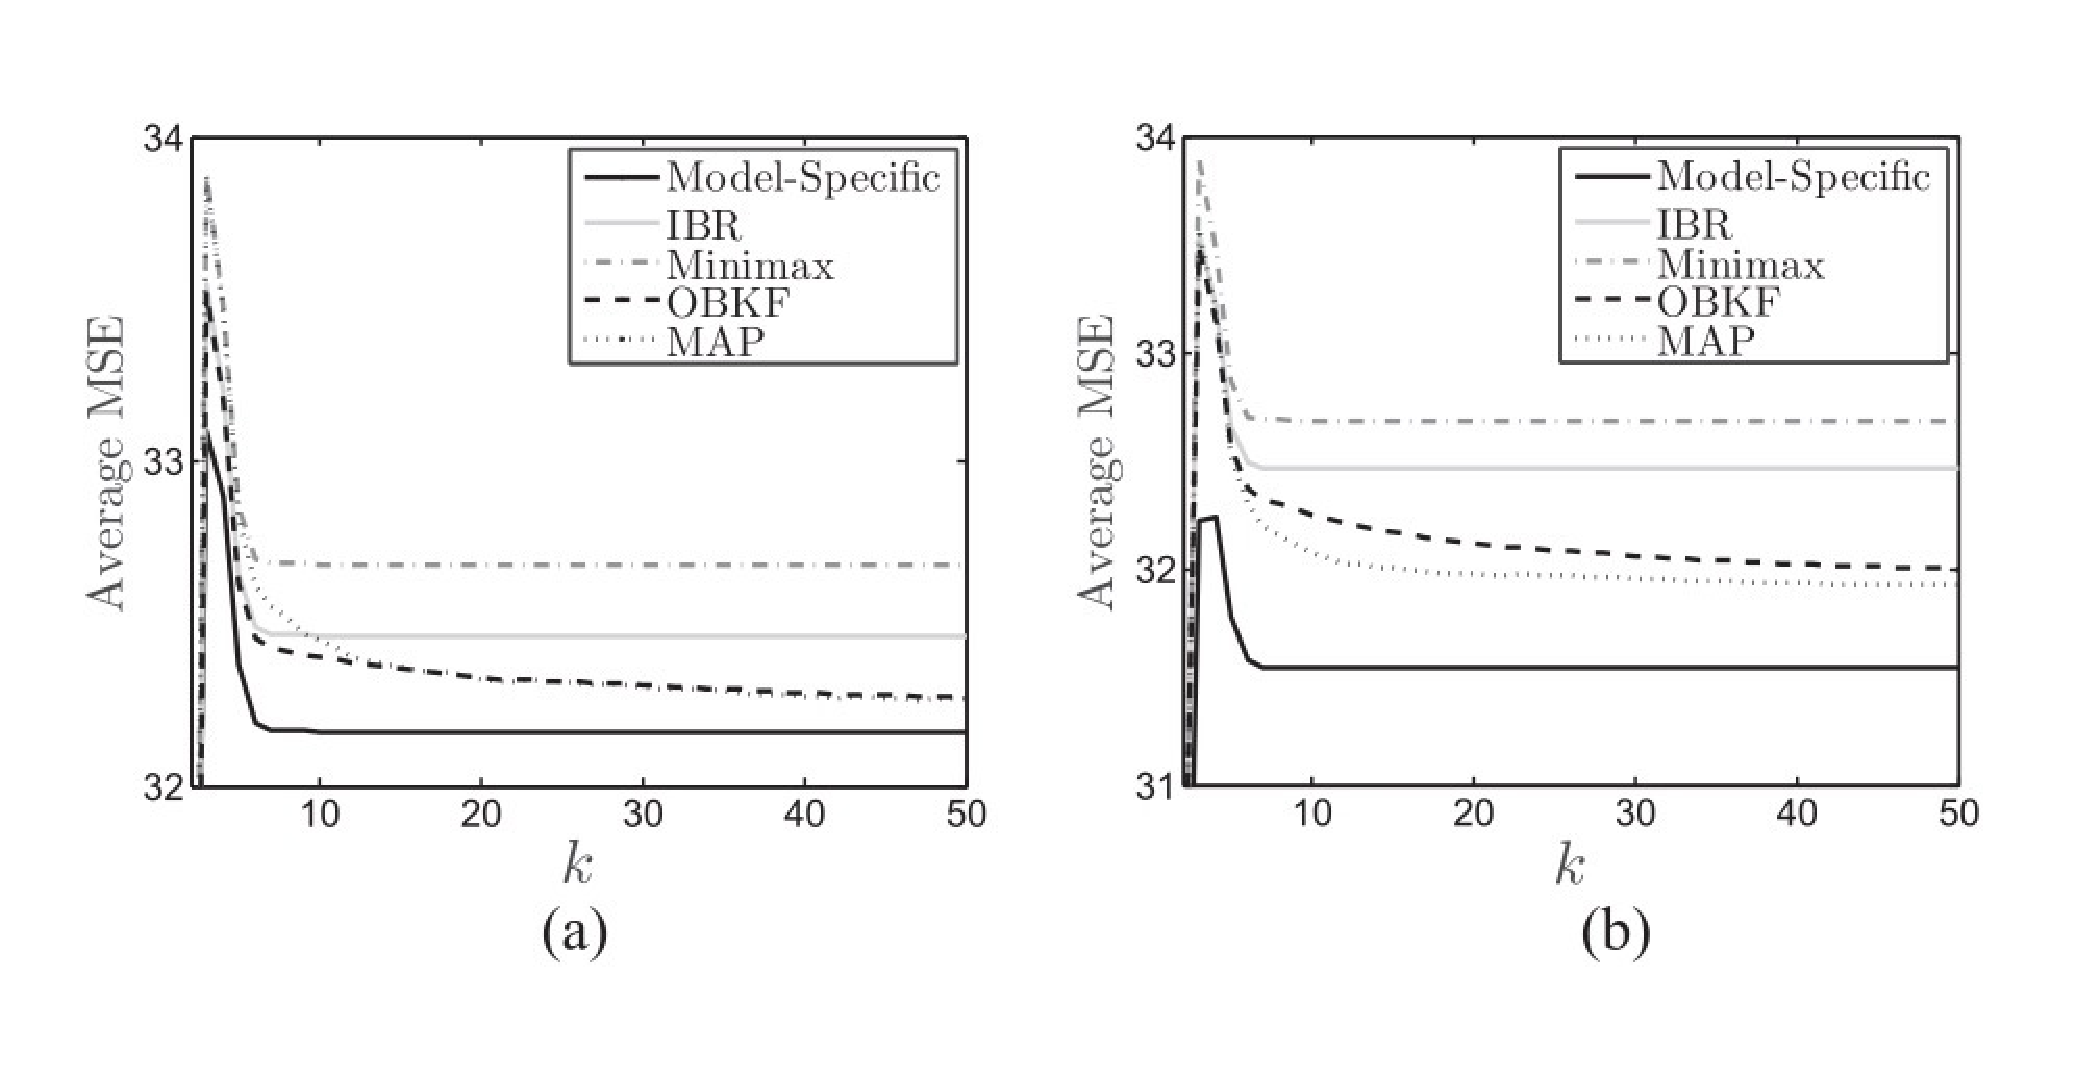
\includegraphics[width=10cm]{img/wrong_prior.eps}
    \caption{Average performance with unknown $r$. The assumed prior distribution is uniform distribution over the interval [3, 6]. (a) True uncertainty interval [2, 7] (b) True uncertainty interval [0.5, 8.5]. Cited from \cite{Dehghannasiri2018}}
    \label{fig:wrong_prior}
    \end{center}
\end{figure}

Although the OBKF is accurate and efficient, the accuracy of the OBKF depends on the prior knowledge. If the true prior distribution is different from the prior distribution in the OBKF, the OBKF doesn't converge to the optimal performance. Fig.\ref{fig:wrong_prior} shows the MSE of the Kalman filters with incorrect prior distribution. Since the prior distribution doesn't include the true value in some simulation, there is a possibility that the OBKF doesn't find the true value. 
\section{Problems and Future Works}
\section{Conclusion and Future Work}\label{sec:conclusion}

The OBKF provides the optimal estimation relative to the posterior distribution. Since it utilizes the prior knowledge, it doesn't require a lot of data compared with the adaptive filter. 
However, the OBKF is computationally expensive. This problem can be solved if the environment is static or the change of the unknown parameter is small. Developing more efficient algorithm is a future work.
Also, if the prior distribution of the OBKF is very different from the true prior distribution, the OBKF doesn't converge to the optimal estimation. This is another drawback of the OBKF.

\bibliographystyle{unsrt}
\bibliography{mybib} 
%----------------------------------------------------------------------------------------

\end{document}